\documentclass[aps,prl,reprint,superscriptaddress,nofootinbib]{revtex4-2}
\usepackage{graphicx}
\usepackage{amsmath}
\usepackage{booktabs}
\usepackage{array}
\usepackage{xcolor}
\begin{document}

\title{A CMS Open Data Diagnostic Search for $H\to\tau\tau$ in the $\mu\tau_h$ Final State}
\author{Analysis my\_analysis}
\affiliation{CMS Open Data reduced-sample analysis}
\date{June 2, 2026}

\begin{abstract}
A diagnostic search for Higgs boson decays to tau pairs is performed with
CMS 2012 Open Data reduced samples in the $\mu\tau_h$ final state.  An
optimized calibrated-score model is trained with multivariate input
reweighting, widened DY/Z normalization, and a same-sign data-driven QCD/fake
template.  The score fit gives
$\mu=38.380^{+7.035}_{-6.116}$
from the profile likelihood and an observed 95\% CLs upper limit
$\mu<50.000$, but it fails the observed validation
gate.  The previous visible-mass result is retained as the validated baseline:
$\mu=0.438^{+4.944}_{-0.438}$, 95\% CLs $\mu<10.764$, exp. $\mu<10.738$.
\end{abstract}

\maketitle

\paragraph{Data and method.}
The analysis uses the public Run2012B/C TauPlusX HiggsTauTauReduced mirror and
the CMS Open Data luminosity reference of 11.467 fb$^{-1}$.  Signal and
background simulations are normalized with official Open Data record event
denominators rather than local reduced-file entries.  Events are selected with
the $\mu+\tau_h$ trigger, tight muon and hadronic-tau requirements including a
tight anti-muon veto, opposite-sign charge, and low transverse mass.

\paragraph{Background correction.}
The W+jets normalization is measured in a high-$m_T$ control region.  The
VBF-background rate is calibrated in a VBF-like top-btag control region outside
the low-$m_T$ signal region, giving a scale
$0.557\pm0.051$.
The reducible QCD/fake contribution is estimated from same-sign low-$m_T$ data
after subtracting non-QCD simulation.  For the primary calibrated-score fit, the
OS/SS transfer factor measured in the lowest score bin is
$0.020\pm0.253$.
The classifier input correction is derived before training from validation and
control regions using a multivariate data-vs-background density-ratio model.
Embedded and EWK $Z$ reduced samples are unavailable, so the DY/Z normalization
is loosened rather than replaced by fabricated samples.

\begin{table}[b]
\caption{Selected yields in the primary calibrated-score fit after the
QCD/fake, DY/Z, and input-reweighting corrections.  Background includes DY,
ttbar, W+jets, and the same-sign QCD/fake estimate.}
\begin{ruledtabular}
\begin{tabular}{lrrrr}
Category & Data & Bkg. & QCD/fake & Signal \\
vbf & 79 & 60.2 & 0.4 & 1.59 \\
boosted & 2213 & 2115.5 & 5.6 & 9.17 \\
zero\_jet & 8466 & 14047.1 & 22.9 & 14.34 \\
\end{tabular}
\end{ruledtabular}
\end{table}

\begin{table*}[t]
\caption{Comparison of the reduced open-data results with published and world
reference context.  The open-data rows use only the localized 2012
$\mu\tau_h$ reduced samples and are not direct reproductions of the
multi-channel CMS or ATLAS+CMS analyses.}
\begin{ruledtabular}
\begin{tabular}{p{0.16\textwidth}p{0.27\textwidth}cp{0.40\textwidth}}
Result & Scope & Significance & Signal-strength information \\
Optimized score attempt & 8 TeV $\mu\tau_h$ reduced, calibrated score & 12.470 & $\mu=38.380^{+7.035}_{-6.116}$, 95\% CLs $\mu<50.000$, exp. $\mu<1.974$, gate fail \\
This analysis baseline & 8 TeV $\mu\tau_h$ reduced, visible mass & 0.095 & $\mu=0.438^{+4.944}_{-0.438}$, 95\% CLs $\mu<10.764$, exp. $\mu<10.738$ \\
CMS Run 1 & 7+8 TeV multi-channel & obs. 3.2, exp. 3.7 & $\mu=0.78\pm0.27$ \\
CMS 2018 & 13 TeV multi-channel & obs. 4.9, exp. 4.7 & $\mu\simeq1.09$ \\
CMS 2018 combined & CMS 7+8+13 TeV & obs. 5.9, exp. 5.9 & CMS combination context \\
ATLAS+CMS Run 1 & 7+8 TeV global Higgs rates & global context & $\mu=1.09\pm0.11$ \\
PDG/HXSWG SM & $H\to\tau\tau$ branching fraction & not a search & BR about 6.3\%, $\mu=1$ convention \\
\end{tabular}
\end{ruledtabular}
\end{table*}

\paragraph{Results.}
The primary corrected workspace has median expected 95\% CLs limit
$\mu<1.974$ and observed limit
$\mu<50.000$.  The best fit is
$\mu=38.380^{+7.035}_{-6.116}$
from the profile likelihood, but it fails the observed validation gate.  The
frozen previous visible-mass baseline gives $\mu=0.438^{+4.944}_{-0.438}$, 95\% CLs $\mu<10.764$, exp. $\mu<10.738$ and is retained as
the validated result for this reduced Open Data workflow.

\begin{figure}[t]
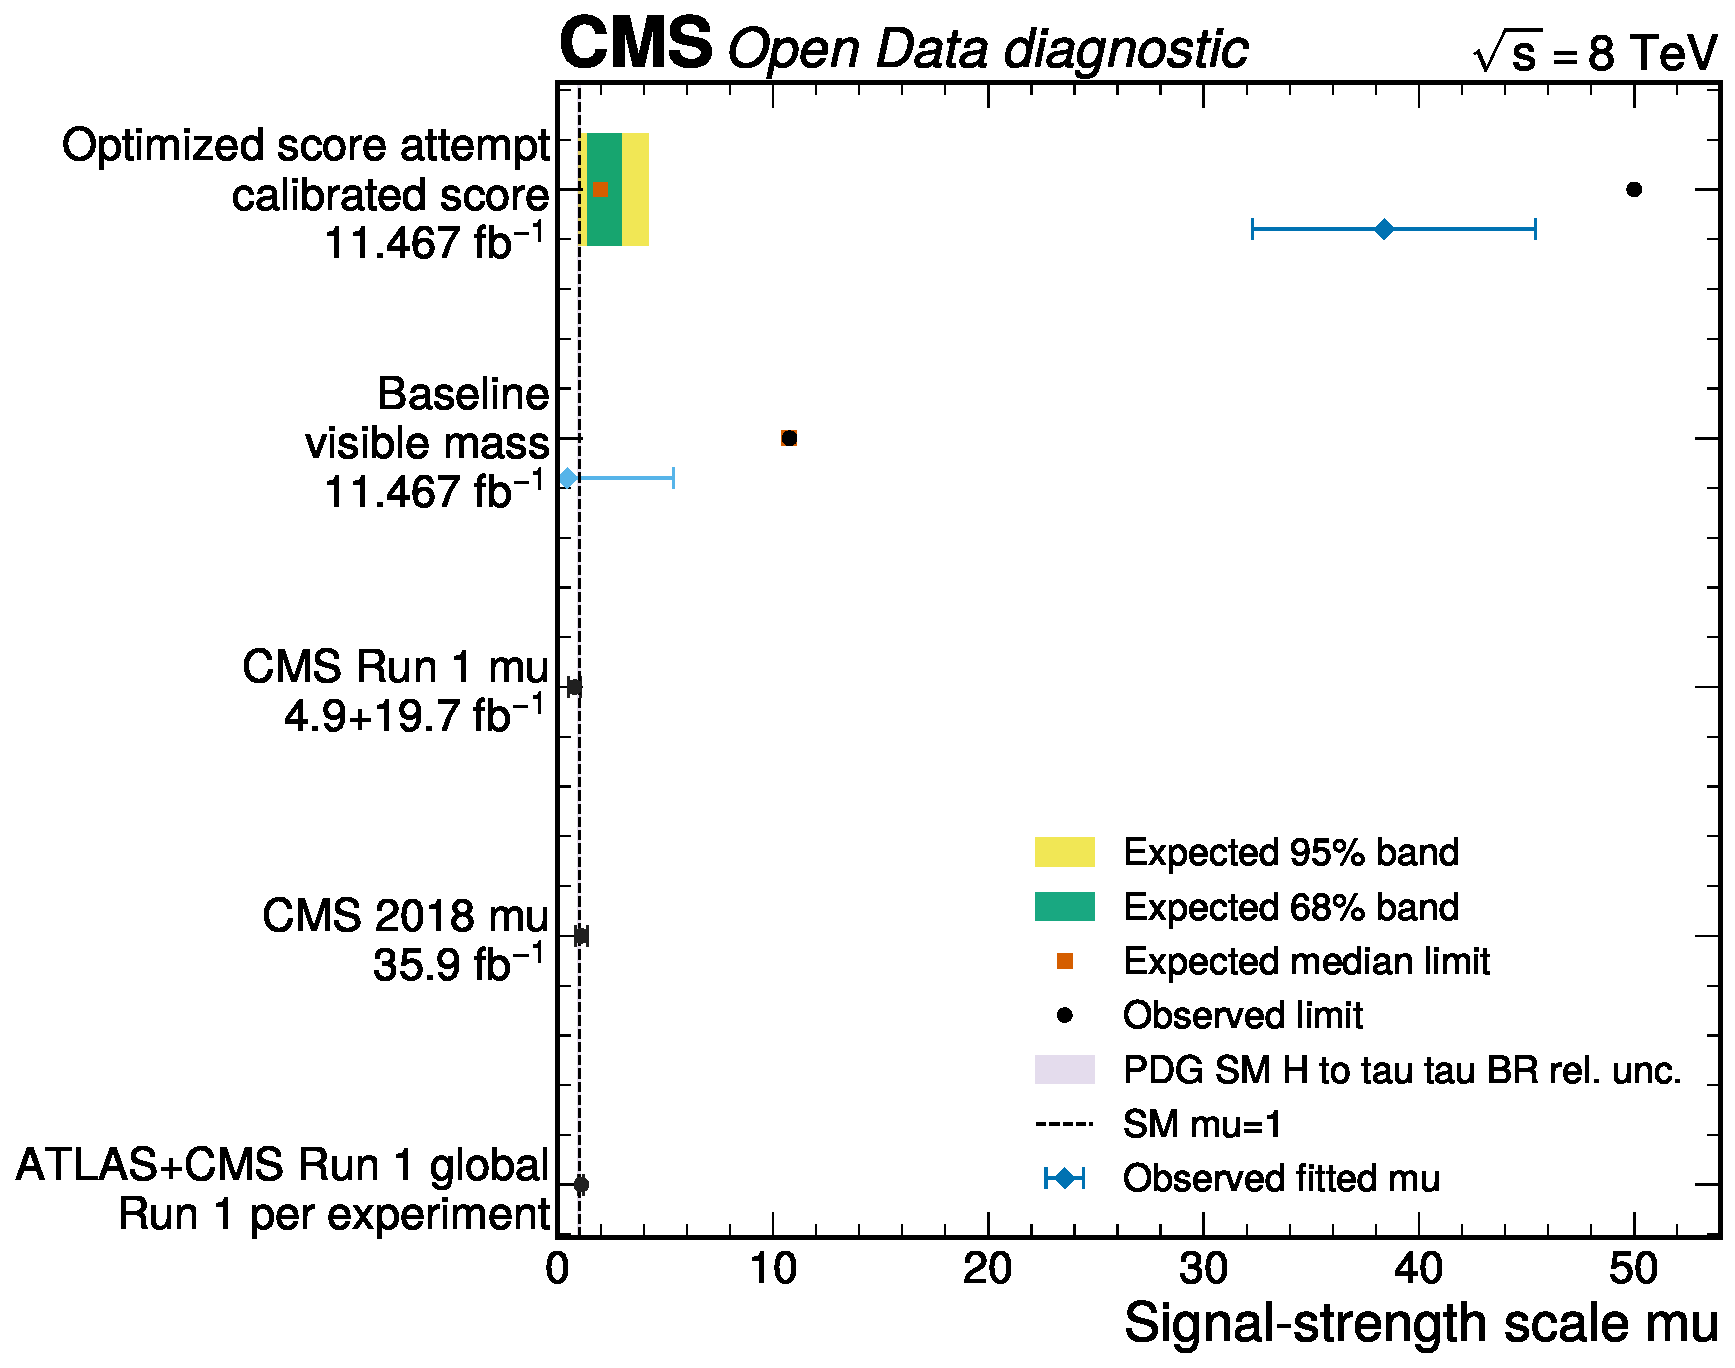
\includegraphics[width=\linewidth]{figures/phase5_mu_limit_comparison.pdf}
\caption{Signal-strength and limit comparison.  The primary open-data result
is shown with expected bands and an observed marker following CMS-style limit
plot conventions.  The CMS/ATLAS+CMS publication rows are context, and the
narrow band at $\mu=1$ shows the PDG/Higgs-summary SM $H\to\tau\tau$
normalization uncertainty.}
\end{figure}

\begin{figure}[t]
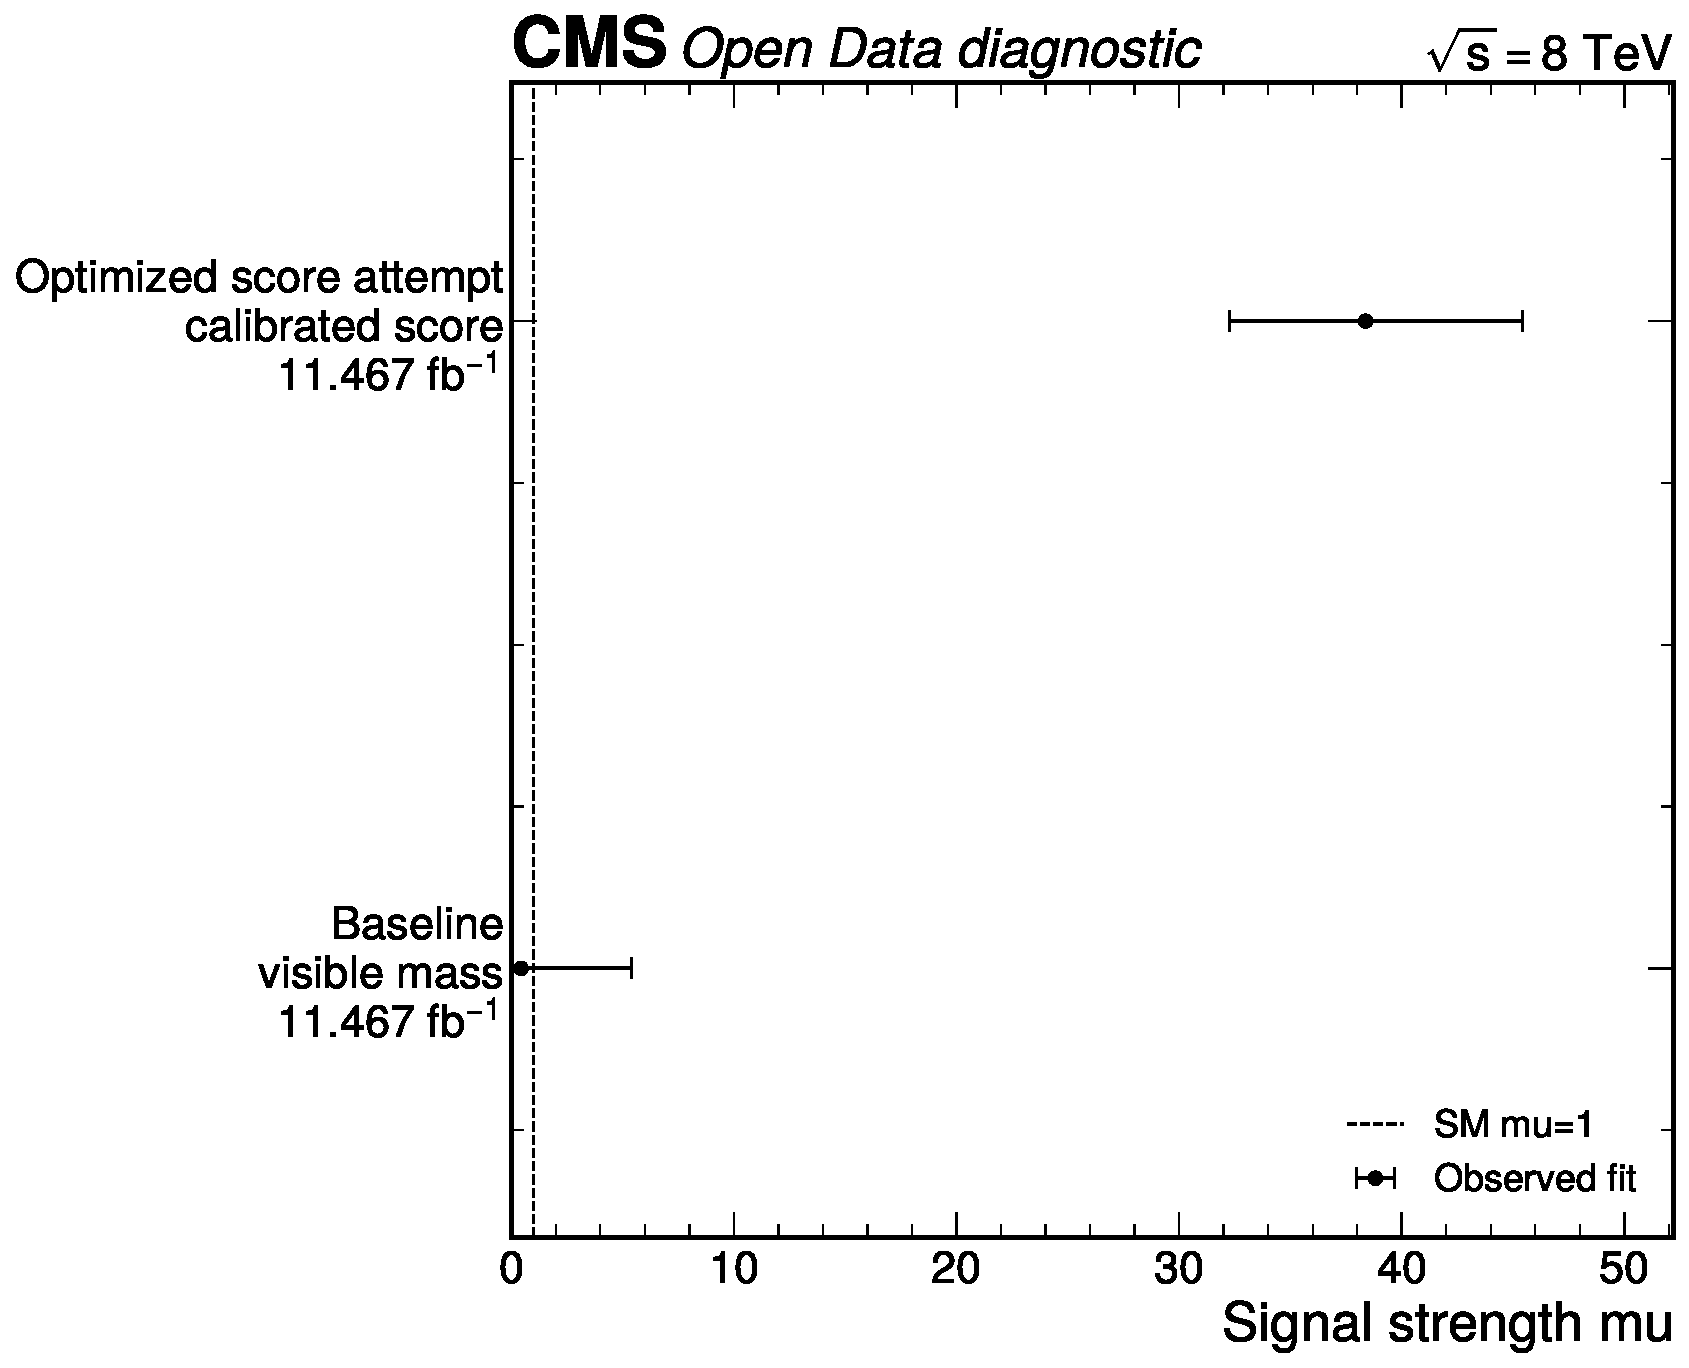
\includegraphics[width=\linewidth]{figures/phase5_primary_vs_baseline_mu.pdf}
\caption{Primary and baseline signal-strength comparison.  The calibrated
score primary result is compared with the frozen previous visible-mass
baseline using profile-likelihood $\mu$ intervals.}
\end{figure}

\begin{figure}[t]
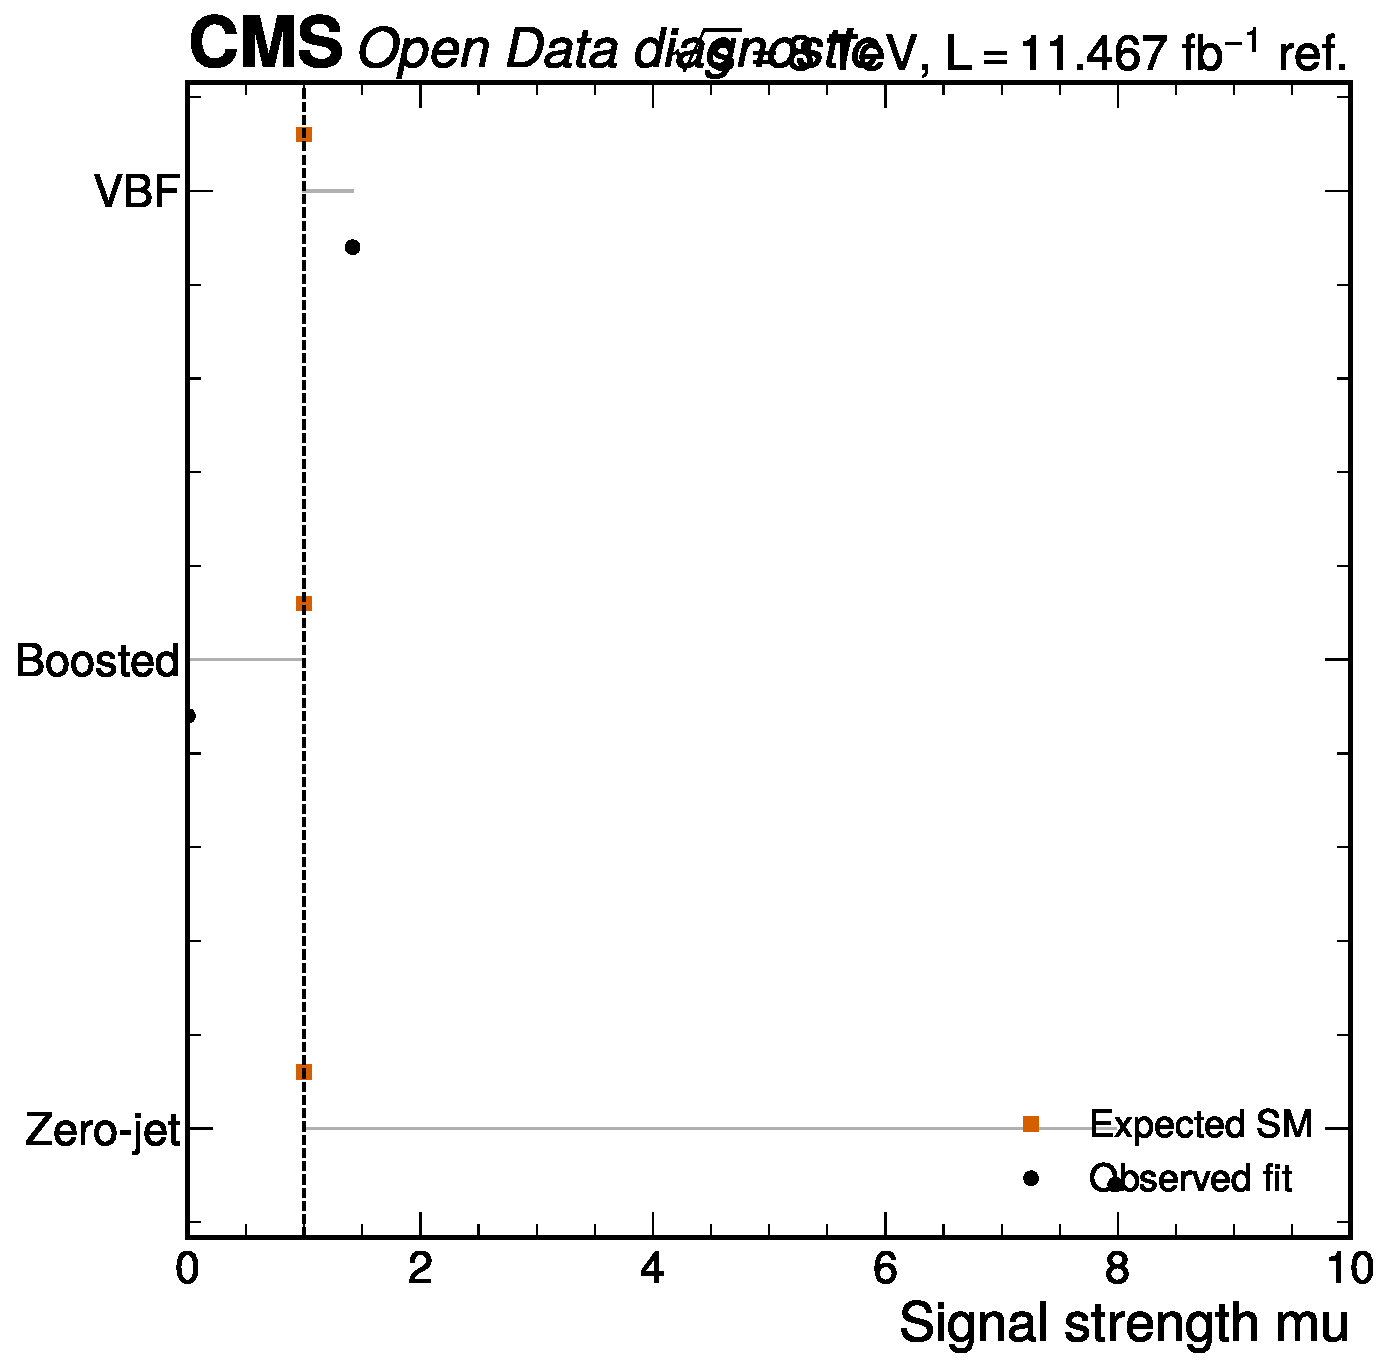
\includegraphics[width=\linewidth]{figures/phase5_category_mu_comparison.pdf}
\caption{Category signal-strength comparison for the primary calibrated-score
model.  The expected marker is the Standard Model value $\mu=1$ and the
observed marker is the single-category profile-fit value; the quoted result
remains the simultaneous three-category fit.}
\end{figure}

\begin{figure}[t]
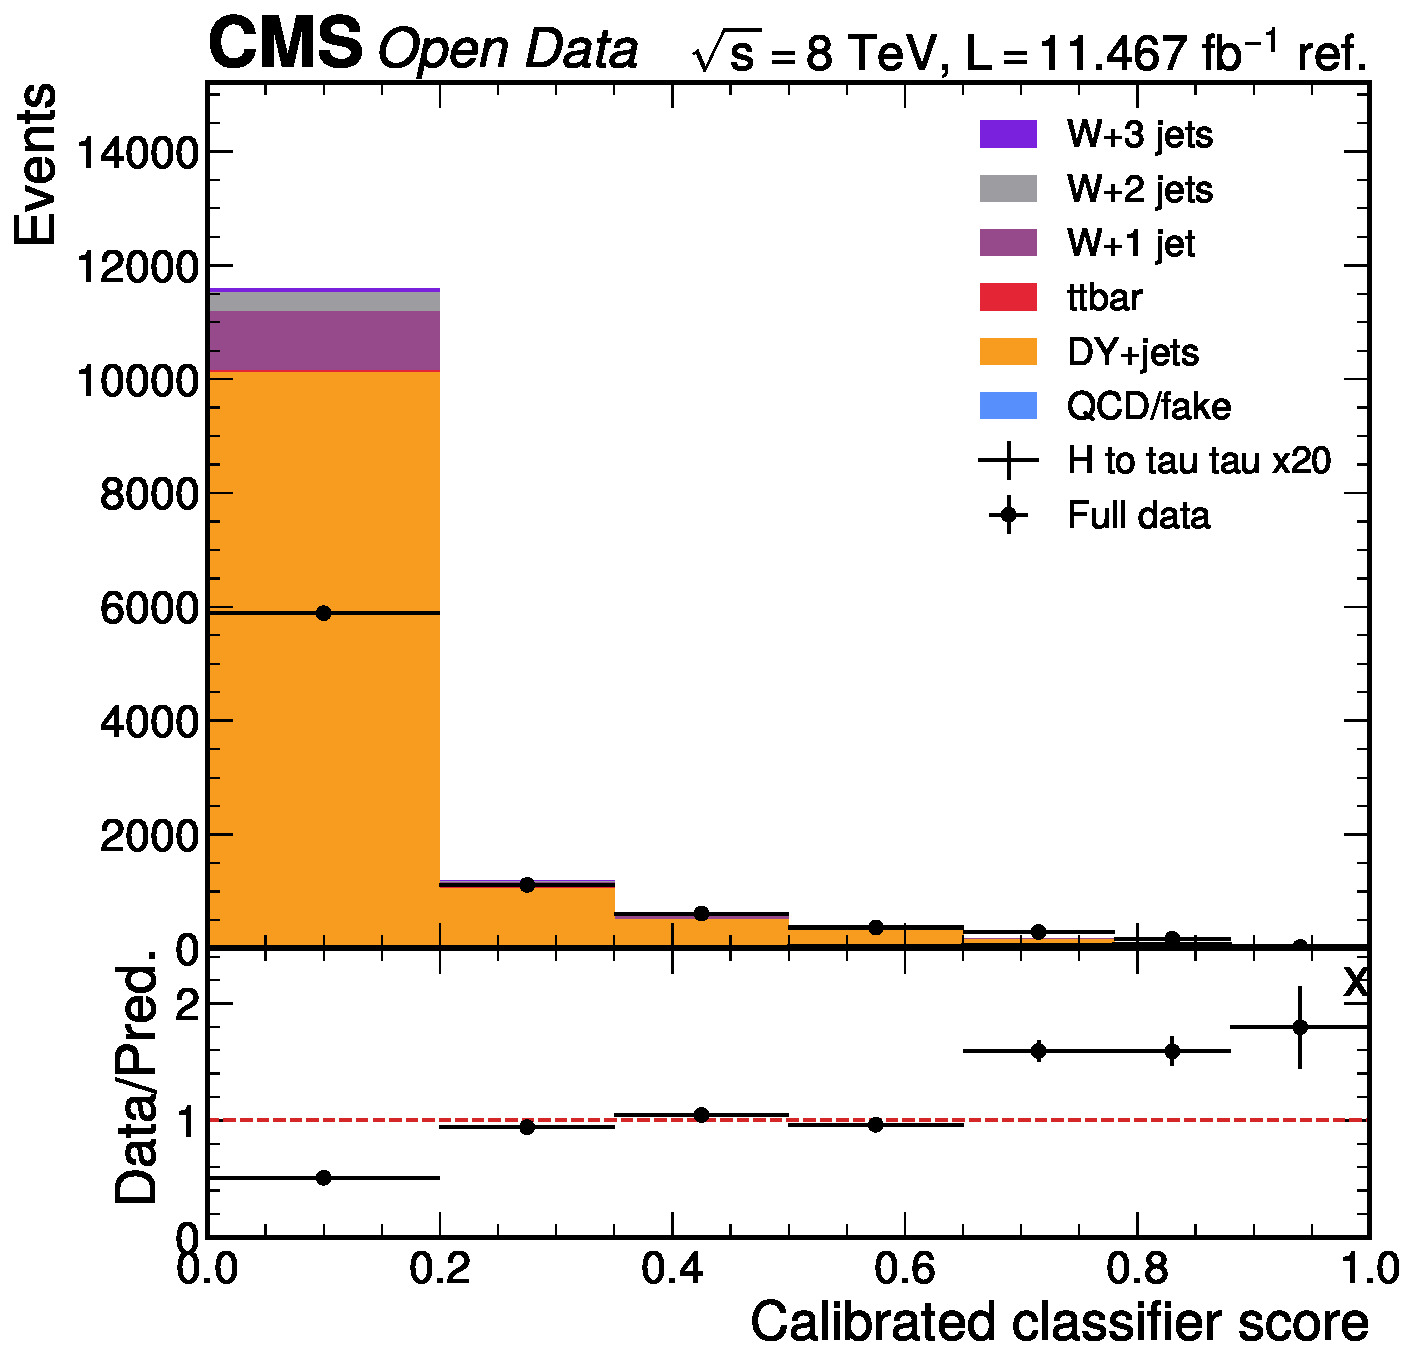
\includegraphics[width=\linewidth]{figures/observed_primary_score_zero_jet.pdf}
\caption{Primary calibrated-score validation in the zero-jet category.  The
same-sign QCD/fake estimate and pre-training input reweighting stabilize the
dominant zero-jet normalization.}
\end{figure}

\paragraph{Comparison and interpretation.}
CMS Run 1 reported evidence for $H\to\tau\tau$ with a best-fit signal strength
of $0.78\pm0.27$ and observed and expected significances of 3.2 and 3.7.  CMS
later observed the decay at 13 TeV with observed and expected significances of
4.9 and 4.7, and reported 5.9 standard deviations in the CMS combination.  The
ATLAS+CMS Run 1 combination and PDG/Higgs-summary branching fraction provide
global context but are not direct validation targets for this reduced
single-channel analysis.  The present result is methodological reproducibility,
not an independent CMS-quality evidence claim.

\begin{thebibliography}{9}
\bibitem{cms2014} CMS Collaboration, Evidence for the 125 GeV Higgs boson decaying to a pair of tau leptons, JHEP 05 (2014) 104.
\bibitem{cms2018} CMS Collaboration, Observation of the SM scalar boson decaying to a pair of tau leptons, Phys. Lett. B 779 (2018) 283.
\bibitem{atlascms2016} ATLAS and CMS Collaborations, Measurements of the Higgs boson production and decay rates and constraints on its couplings from a combined ATLAS and CMS analysis, JHEP 08 (2016) 045.
\bibitem{pdg2024} Particle Data Group, Review of Particle Physics, Phys. Rev. D 110 (2024) 030001.
\bibitem{opendata} CERN Open Data Portal, CMS Higgs to tau tau reduced samples for education and outreach.
\bibitem{pyhf} L. Heinrich et al., pyhf: pure-Python implementation of HistFactory statistical models.
\bibitem{cls} A. L. Read, Presentation of search results: the CLs technique.
\bibitem{cowan} G. Cowan et al., Asymptotic formulae for likelihood-based tests of new physics.
\end{thebibliography}

\end{document}
